\section{Supporting Information: PDIpy}

\subsection{Molecular Orbitals}
The electronic difference between $^1\Delta_g$ and $^3\Sigma_g^-$ is best depicted through their respective molecular orbital diagrams in Figure \ref{mo_diagrams}.

\begin{figure}
    \centering
    \begin{tabular}{c|c}
        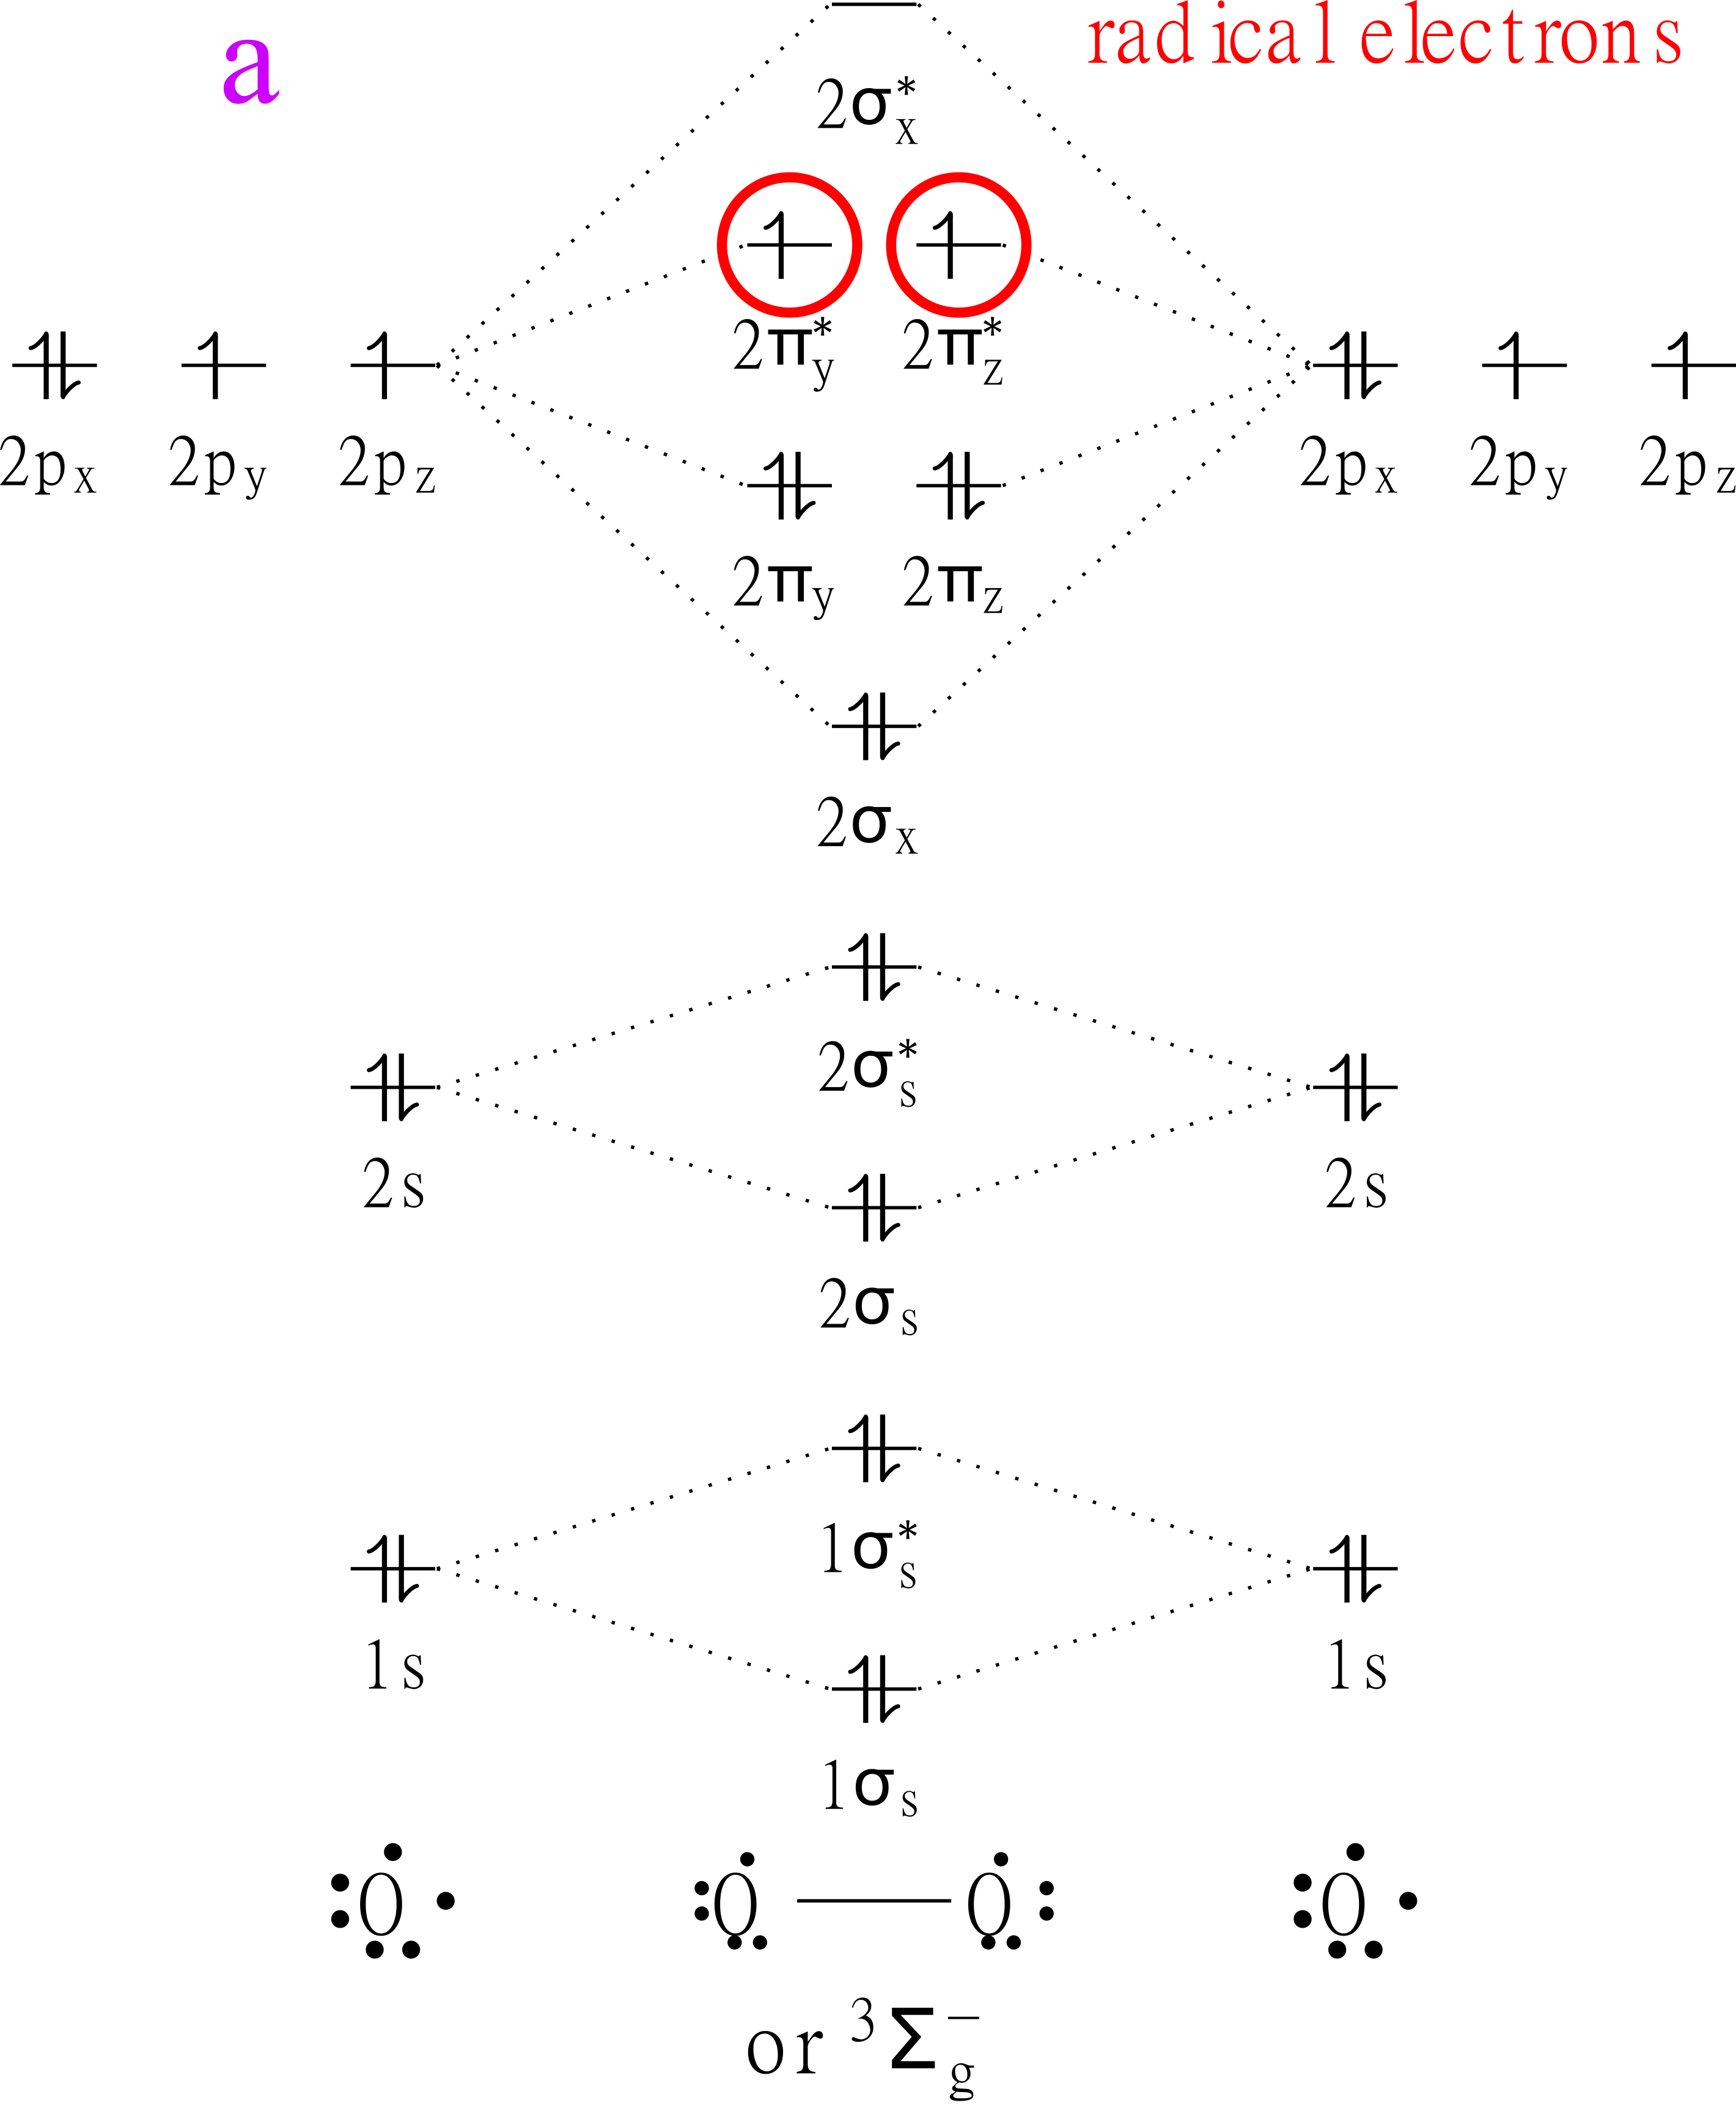
\includegraphics[width = 0.48\textwidth]{images/background/triplet_mo_diagram.png}
        & 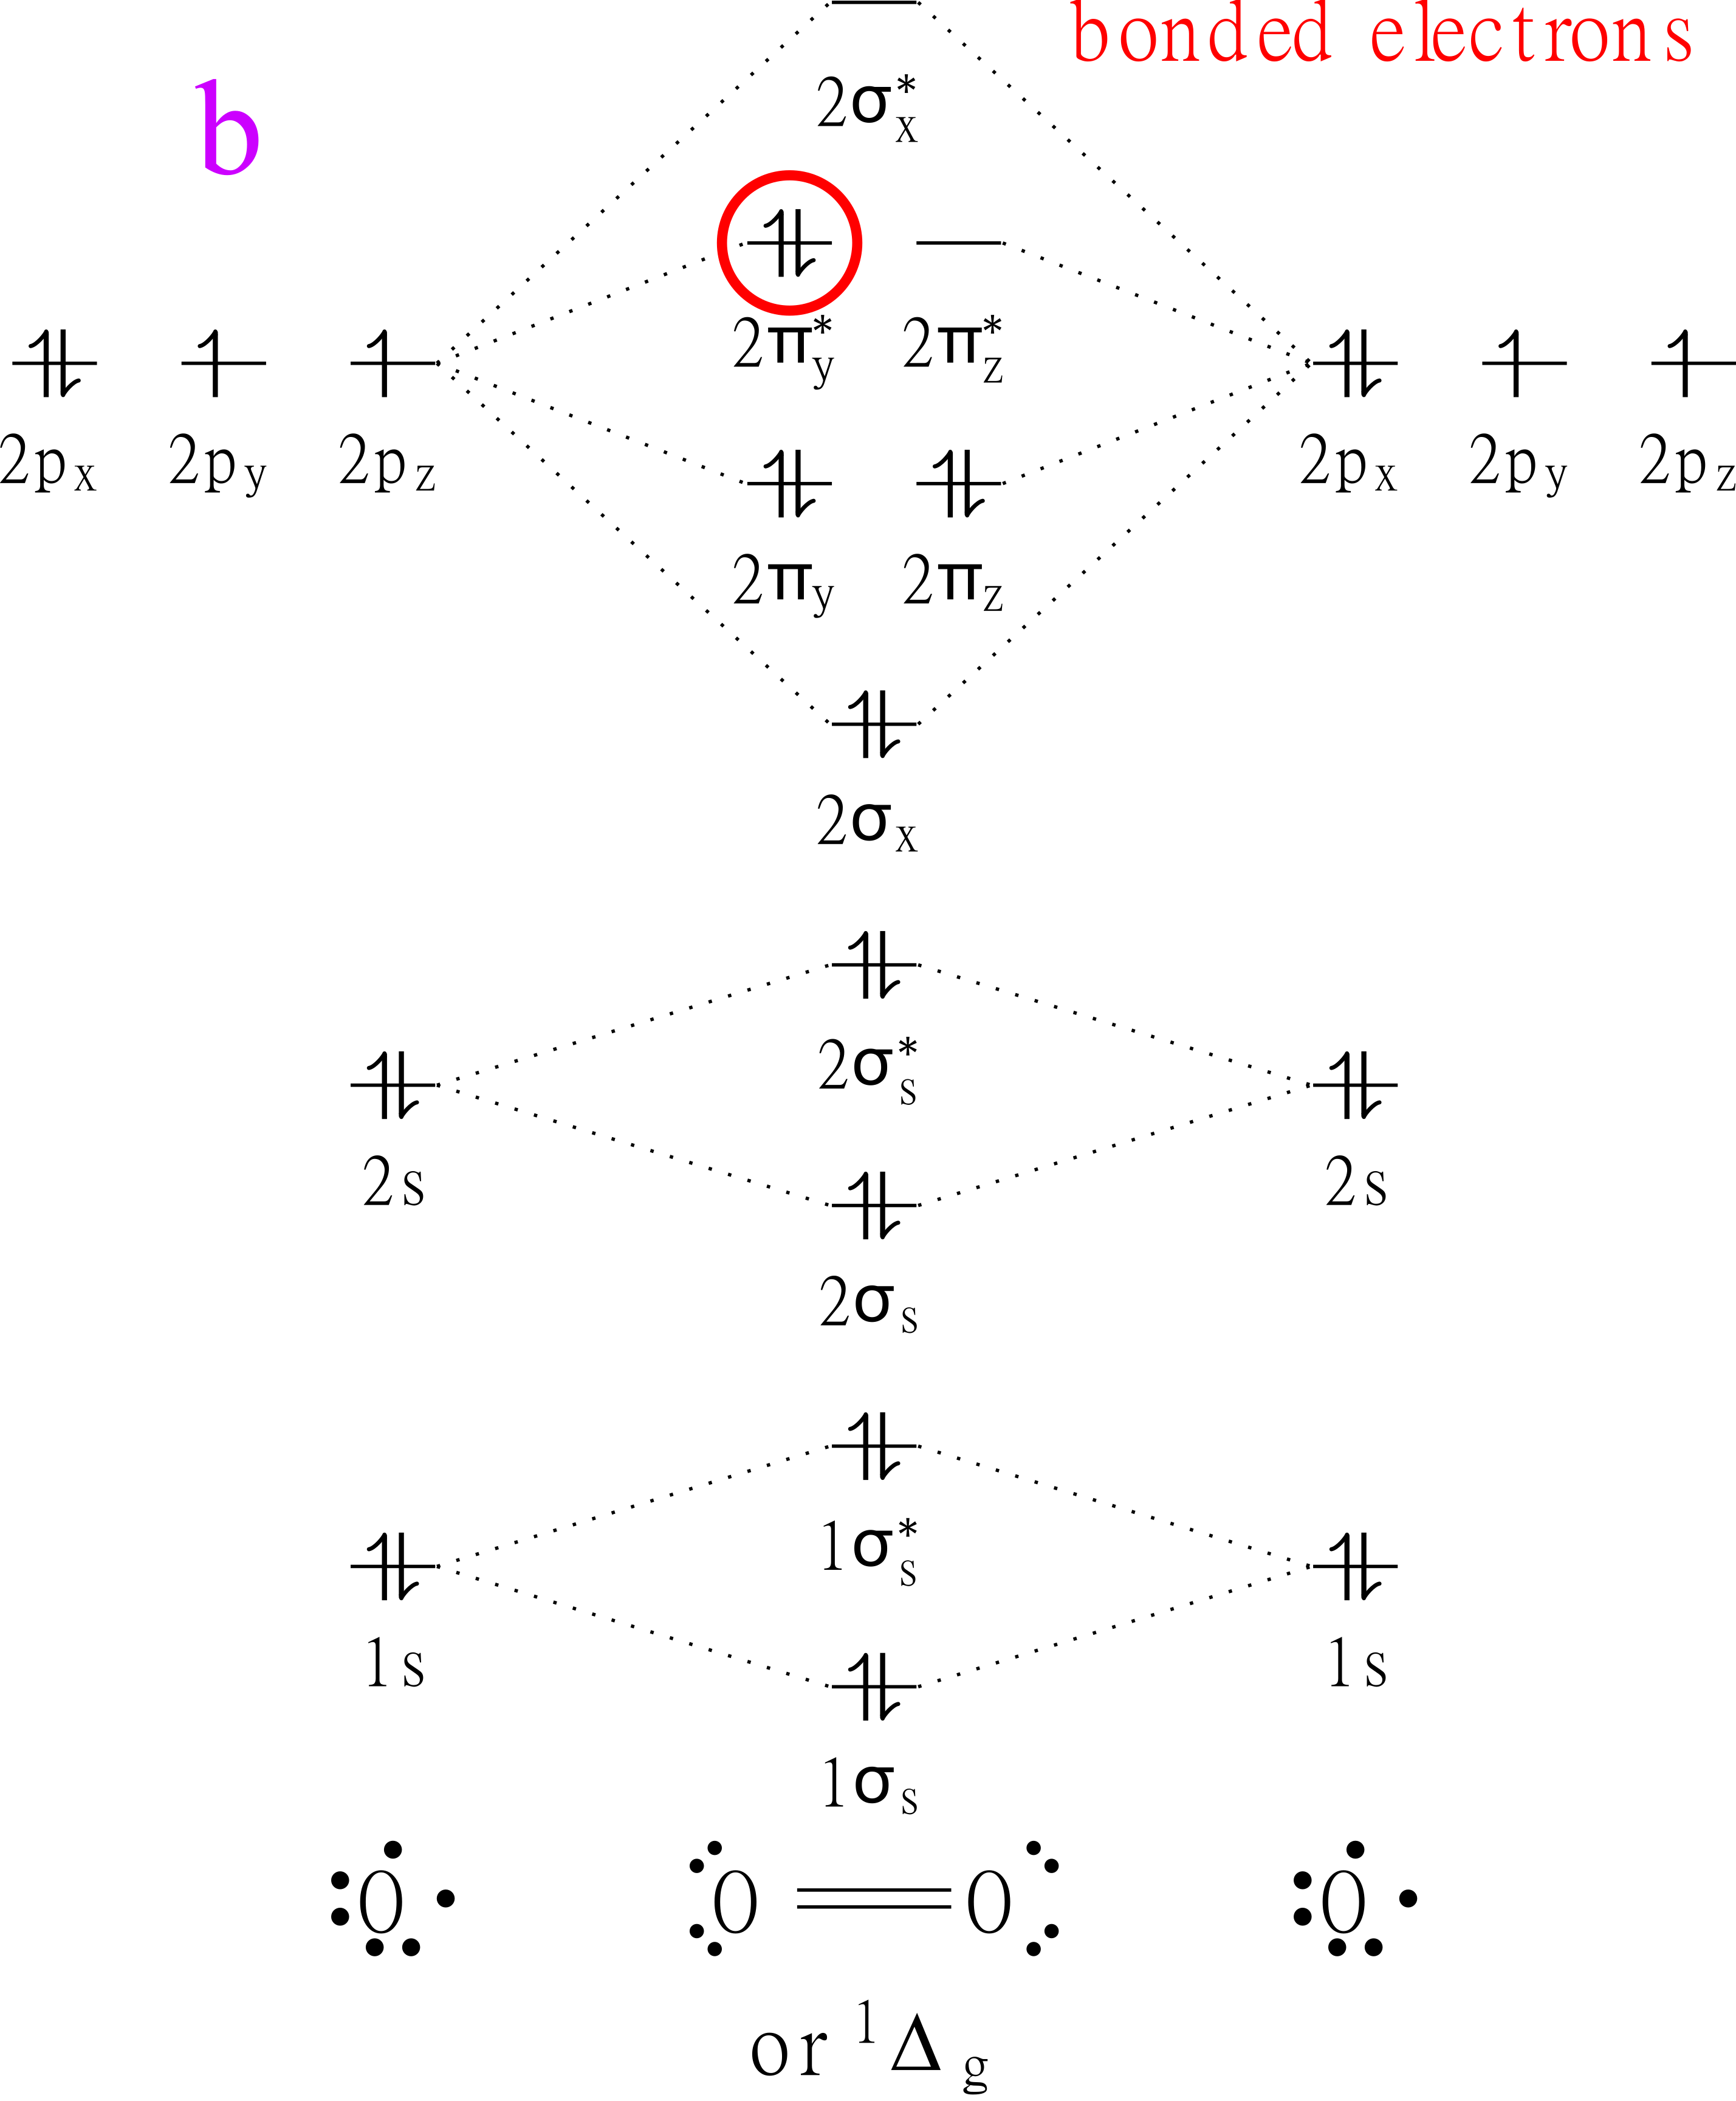
\includegraphics[width = 0.48\textwidth]{images/background/singlet_mo_diagram.png}
    \end{tabular}
    \caption{
        Qualitative orbital diagrams for diatomic oxygen. Each barbed arrows represent single electron, and each platform represents the electronic orbital of the respective label. Panel a) depicts the ground triplet state ($^3\Sigma_g^-$), which characteristically contains two radical electrons in its highest occupied molecular orbital (HOMO). Panel b) depicts the excited singlet state ($^1\Delta_g$), which characteristically contains a $\pi^*$-bond in its HOMO that destabilizes the molecule and contributes to greater reactivity.
    }
    \label{mo_diagrams}
\end{figure}


\subsection{Oxidized membrane region}
The region of the bacterial membrane that is oxidized by PDI systems with cross-linked PSs may be a small fraction of the total membrane, provided that the bacterium does not have a tremendous angular momentum. This is the consequence of the stationary PS on one side of the bacterium, unlike dissolved PSs that encapsulate the simulated bacterium and thereby oxidize it from all sides. The oxidized region of a coccus bacterial cell can be determined from the cellular radius and volume
\begin{equation}
    radius_{cell} = \sqrt[3]{3*\frac{volume_{cell}}{4\pi}}~,
\end{equation}
where the volume is often reported in literature. The membrane volume 
\begin{equation}
    volume_{membrane} = \frac{4\pi}{3}*(radius_{cell}^3* - (radius_{cell}-th_{membrane})^3)
\end{equation}
can be calculated with knowledge of the thickness of the cytoplasmic membrane, which is $\approx 4 nm$. The volume of oxidized membrane is then calculated
\begin{equation}
    volume_{oxidized} = \frac{2\pi}{3}*(1-angle_{oxidized})\\ 
        *(radius_{cell}^3* - (radius_{cell}-th_{membrane})^3)~,    
\end{equation}
where the $angle_{oxidized}$ describes the angle from vertical at which the farthest $^1\Delta_g$ reaches the mebrane. This is conceptually similar to the $angle_{absorption}$ from the thermodynamic metabolism from the Supporting Information of the WCMpy chapter. The fraction of the membrane volume that is oxidized is then calculated 
\begin{equation}
    oxidized = \frac{volume_{oxidized}}{volume_{membrane}} 
\end{equation}
and applied to augment the effective oxidation proportion from \cref{oxidation_proportion}
\begin{equation}
    oxidation_{proportion,new} = \frac{oxidation_{proportion,old}}{oxidized}~.
\end{equation}
